% Options for packages loaded elsewhere
\PassOptionsToPackage{unicode}{hyperref}
\PassOptionsToPackage{hyphens}{url}
%
\documentclass[
  12pt,
]{article}
\usepackage{amsmath,amssymb}
\usepackage{lmodern}
\usepackage{iftex}
\ifPDFTeX
  \usepackage[T1]{fontenc}
  \usepackage[utf8]{inputenc}
  \usepackage{textcomp} % provide euro and other symbols
\else % if luatex or xetex
  \usepackage{unicode-math}
  \defaultfontfeatures{Scale=MatchLowercase}
  \defaultfontfeatures[\rmfamily]{Ligatures=TeX,Scale=1}
  \setmainfont[]{Times New Roman}
\fi
% Use upquote if available, for straight quotes in verbatim environments
\IfFileExists{upquote.sty}{\usepackage{upquote}}{}
\IfFileExists{microtype.sty}{% use microtype if available
  \usepackage[]{microtype}
  \UseMicrotypeSet[protrusion]{basicmath} % disable protrusion for tt fonts
}{}
\makeatletter
\@ifundefined{KOMAClassName}{% if non-KOMA class
  \IfFileExists{parskip.sty}{%
    \usepackage{parskip}
  }{% else
    \setlength{\parindent}{0pt}
    \setlength{\parskip}{6pt plus 2pt minus 1pt}}
}{% if KOMA class
  \KOMAoptions{parskip=half}}
\makeatother
\usepackage{xcolor}
\usepackage[margin=2.54cm]{geometry}
\usepackage{color}
\usepackage{fancyvrb}
\newcommand{\VerbBar}{|}
\newcommand{\VERB}{\Verb[commandchars=\\\{\}]}
\DefineVerbatimEnvironment{Highlighting}{Verbatim}{commandchars=\\\{\}}
% Add ',fontsize=\small' for more characters per line
\usepackage{framed}
\definecolor{shadecolor}{RGB}{248,248,248}
\newenvironment{Shaded}{\begin{snugshade}}{\end{snugshade}}
\newcommand{\AlertTok}[1]{\textcolor[rgb]{0.94,0.16,0.16}{#1}}
\newcommand{\AnnotationTok}[1]{\textcolor[rgb]{0.56,0.35,0.01}{\textbf{\textit{#1}}}}
\newcommand{\AttributeTok}[1]{\textcolor[rgb]{0.77,0.63,0.00}{#1}}
\newcommand{\BaseNTok}[1]{\textcolor[rgb]{0.00,0.00,0.81}{#1}}
\newcommand{\BuiltInTok}[1]{#1}
\newcommand{\CharTok}[1]{\textcolor[rgb]{0.31,0.60,0.02}{#1}}
\newcommand{\CommentTok}[1]{\textcolor[rgb]{0.56,0.35,0.01}{\textit{#1}}}
\newcommand{\CommentVarTok}[1]{\textcolor[rgb]{0.56,0.35,0.01}{\textbf{\textit{#1}}}}
\newcommand{\ConstantTok}[1]{\textcolor[rgb]{0.00,0.00,0.00}{#1}}
\newcommand{\ControlFlowTok}[1]{\textcolor[rgb]{0.13,0.29,0.53}{\textbf{#1}}}
\newcommand{\DataTypeTok}[1]{\textcolor[rgb]{0.13,0.29,0.53}{#1}}
\newcommand{\DecValTok}[1]{\textcolor[rgb]{0.00,0.00,0.81}{#1}}
\newcommand{\DocumentationTok}[1]{\textcolor[rgb]{0.56,0.35,0.01}{\textbf{\textit{#1}}}}
\newcommand{\ErrorTok}[1]{\textcolor[rgb]{0.64,0.00,0.00}{\textbf{#1}}}
\newcommand{\ExtensionTok}[1]{#1}
\newcommand{\FloatTok}[1]{\textcolor[rgb]{0.00,0.00,0.81}{#1}}
\newcommand{\FunctionTok}[1]{\textcolor[rgb]{0.00,0.00,0.00}{#1}}
\newcommand{\ImportTok}[1]{#1}
\newcommand{\InformationTok}[1]{\textcolor[rgb]{0.56,0.35,0.01}{\textbf{\textit{#1}}}}
\newcommand{\KeywordTok}[1]{\textcolor[rgb]{0.13,0.29,0.53}{\textbf{#1}}}
\newcommand{\NormalTok}[1]{#1}
\newcommand{\OperatorTok}[1]{\textcolor[rgb]{0.81,0.36,0.00}{\textbf{#1}}}
\newcommand{\OtherTok}[1]{\textcolor[rgb]{0.56,0.35,0.01}{#1}}
\newcommand{\PreprocessorTok}[1]{\textcolor[rgb]{0.56,0.35,0.01}{\textit{#1}}}
\newcommand{\RegionMarkerTok}[1]{#1}
\newcommand{\SpecialCharTok}[1]{\textcolor[rgb]{0.00,0.00,0.00}{#1}}
\newcommand{\SpecialStringTok}[1]{\textcolor[rgb]{0.31,0.60,0.02}{#1}}
\newcommand{\StringTok}[1]{\textcolor[rgb]{0.31,0.60,0.02}{#1}}
\newcommand{\VariableTok}[1]{\textcolor[rgb]{0.00,0.00,0.00}{#1}}
\newcommand{\VerbatimStringTok}[1]{\textcolor[rgb]{0.31,0.60,0.02}{#1}}
\newcommand{\WarningTok}[1]{\textcolor[rgb]{0.56,0.35,0.01}{\textbf{\textit{#1}}}}
\usepackage{longtable,booktabs,array}
\usepackage{calc} % for calculating minipage widths
% Correct order of tables after \paragraph or \subparagraph
\usepackage{etoolbox}
\makeatletter
\patchcmd\longtable{\par}{\if@noskipsec\mbox{}\fi\par}{}{}
\makeatother
% Allow footnotes in longtable head/foot
\IfFileExists{footnotehyper.sty}{\usepackage{footnotehyper}}{\usepackage{footnote}}
\makesavenoteenv{longtable}
\usepackage{graphicx}
\makeatletter
\def\maxwidth{\ifdim\Gin@nat@width>\linewidth\linewidth\else\Gin@nat@width\fi}
\def\maxheight{\ifdim\Gin@nat@height>\textheight\textheight\else\Gin@nat@height\fi}
\makeatother
% Scale images if necessary, so that they will not overflow the page
% margins by default, and it is still possible to overwrite the defaults
% using explicit options in \includegraphics[width, height, ...]{}
\setkeys{Gin}{width=\maxwidth,height=\maxheight,keepaspectratio}
% Set default figure placement to htbp
\makeatletter
\def\fps@figure{htbp}
\makeatother
\setlength{\emergencystretch}{3em} % prevent overfull lines
\providecommand{\tightlist}{%
  \setlength{\itemsep}{0pt}\setlength{\parskip}{0pt}}
\setcounter{secnumdepth}{5}
\ifLuaTeX
  \usepackage{selnolig}  % disable illegal ligatures
\fi
\IfFileExists{bookmark.sty}{\usepackage{bookmark}}{\usepackage{hyperref}}
\IfFileExists{xurl.sty}{\usepackage{xurl}}{} % add URL line breaks if available
\urlstyle{same} % disable monospaced font for URLs
\hypersetup{
  pdftitle={Analyzing Soil Moisture \& Precipitation Trends in Coweeta Basin LTER Site},
  pdfauthor={Kelly Davidson, Megan McClaugherty, \& Isabel Zungailia},
  hidelinks,
  pdfcreator={LaTeX via pandoc}}

\title{Analyzing Soil Moisture \& Precipitation Trends in Coweeta Basin
LTER Site}
\usepackage{etoolbox}
\makeatletter
\providecommand{\subtitle}[1]{% add subtitle to \maketitle
  \apptocmd{\@title}{\par {\large #1 \par}}{}{}
}
\makeatother
\subtitle{\url{https://github.com/ibz24/Zungailia_Davidson_McClaugherty}}
\author{Kelly Davidson, Megan McClaugherty, \& Isabel Zungailia}
\date{}

\begin{document}
\maketitle

\newpage
\tableofcontents 
\newpage
\listoftables 
\newpage
\listoffigures 
\newpage

\hypertarget{rationale-and-research-questions}{%
\section{Rationale and Research
Questions}\label{rationale-and-research-questions}}

The Coweeta Basin Long Term Ecological Research (LTER) site is deemed
one of the oldest continuous environmental studies in North America. It
is managed by the USDA Forest Service in collaboration with the
University of Georgia. This site is located in the southern portion of
the Appalachian Mountains in North Carolina and is primarily composed of
deciduous forest. We decided to use this site for our research project
because it provides a unique setting to explore the relationships
between environmental variables such as soil moisture, precipitation,
and elevation over time. The goal of this analysis was to use skills
that we have learned throughout the semester to generate and answer a
specific research question. This investigation was intended to analyze
temporal trends in soil moisture throughout the Coweeta Basin, and we
used soil moisture data from four sites (at four different elevations)
to explore our research questions. We also investigated the relationship
between precipitation and soil moisture over time, assuming that there
is a positive relationship between these two variables. The analysis is
based on data collected between the years 2000 and 2013. The four sites
where soil moisture data was collected are located at four different
elevations, allowing us to infer the relationship between soil moisture
and elevation. The research sites are located at the following
elevations:

\begin{itemize}
\tightlist
\item
  Site 1: 817.17 meters
\item
  Site 2: 1380.44 meters
\item
  Site 3: 1214.93 meters
\item
  Site 4: 735.47 meters
\end{itemize}

The Coweeta LTER laboratory collects precipitation data from a total of
eight rain gauges throughout the Coweeta Basin, so we used the
geographic coordinates of the rain gauges and the four research sites to
determine which rain gauge was located closest to each site. The
precipitation data from Rain Gauge 6 (RG06) was used for Sites 1 and 4,
data from Rain Gauge 31 (RG31) was used for Site 2, and data from Rain
Gauge 5 (RG05) was used for Site 3. All of the sites are within 0.8 km
of their paired rain gauge.

Our main research question: \emph{Has soil moisture in the upper 30 cm
(of soil) increased or decreased in Coweeta Basin from 2000 to 2013 at
each of the four research sites?}

Other questions that were explored include:

\begin{itemize}
\tightlist
\item
  \emph{Which sites experienced the greatest change in soil moisture
  over time?}
\item
  \emph{What is the impact of elevation on soil moisture?}
\item
  \emph{Is there a relationship between soil moisture and precipitation
  that can be observed at these four study sites?}
\end{itemize}

\textbf{Null Hypothesis A}: There was no change in soil moisture in the
upper 30 cm from 2000 to 2013 at each of the four research sites.

\textbf{Alternative Hypothesis A}: There was a change in soil moisture
in the upper 30 cm from 2000 to 2013 at each of the four research sites.

\textbf{Null Hypothesis B}: There is no relationship between soil
moisture and precipitation at each of the four research sites.

\textbf{Alternative Hypothesis B}: There is a relationship between soil
moisture and precipitation at each of the four research sites.

\begin{figure}
\centering
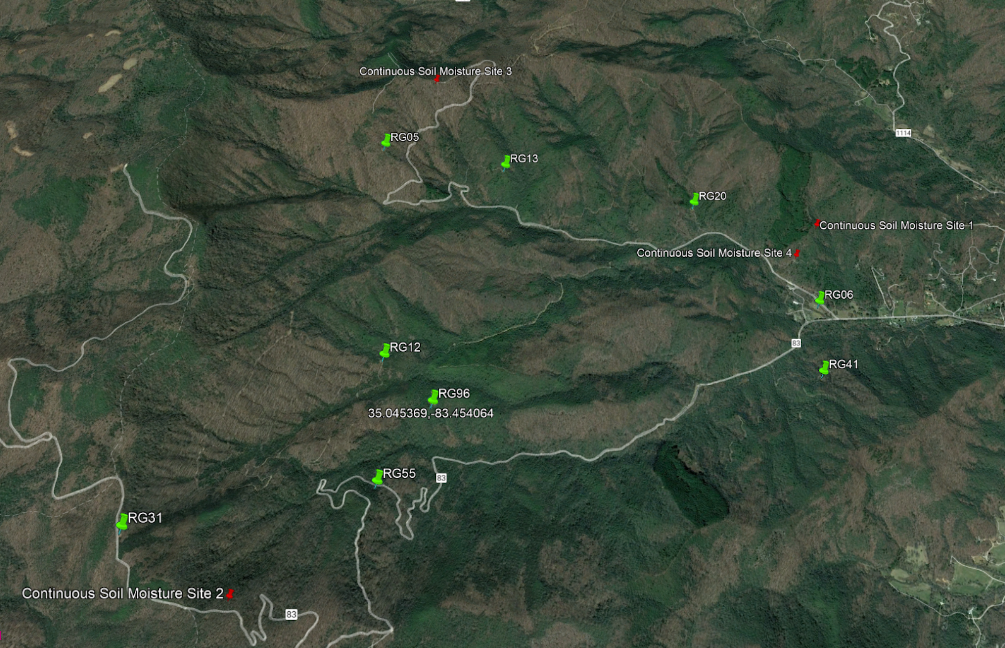
\includegraphics{../Data/precipandsmois.png}
\caption{Soil moisture research sites and rain gauge locations within
Coweeta Basin, North Carolina.}
\end{figure}

\newpage

\hypertarget{dataset-information}{%
\section{Dataset Information}\label{dataset-information}}

\textbf{Data Description}

Soil moisture datasets were collected from the EDI Data Portal for
Coweeta LTER \href{https://portal.edirepository.org/nis/home.jsp}{here}.
Coweeta LTER (248) was selected as the LTER Site and ``Continuously
measured forest soil moisture at four sites in the Coweeta Basin'' was
identified as the dataset of interest. The data was accessed on
11/21/22. The following datasets were downloaded:

\begin{itemize}
\tightlist
\item
  1040\_2000\_2014
\item
  1040.kml (a Google Earth file showing the soil moisture site
  locations)
\end{itemize}

Precipitation data was collected from the US Forest Service Southern
Research Station
\href{https://www.srs.fs.usda.gov/coweeta/tools-and-data/}{here}. Daily
precipitation data from recording rain gages (RRG) at Coweeta Hydrologic
Lab, North Carolina was selected under Coweeta Datasets on the USFS
Research Data Archive
\href{https://www.fs.usda.gov/rds/archive/Catalog/RDS-2017-0031}{here}.
The data was accessed on 11/30/22.

We generated four new datasets combining the monthly average
precipitation with monthly average 30 cm soil moisture at the 4 sites
monitored at the Coweeta LTER.

\textbf{Data Wrangling}

The initial datasets required a significant amount of wrangling before
they could be used for analysis. The raw soil moisture data had 21
variables/columns, so the first step was to select the columns of
interest (site, Year, YearDay, smois30). A new `Date' column was created
(format = ``\%Y-\%j'') and the data was filtered to exclude the smois30
values less than 0 and greater than 1 since soil moisture was expressed
as percent water content. All NAs were omitted from the data and it was
then split into 4 separate dataframes, one for each research site. The
smois30 (cm) values were averaged per month for each site prior to
analysis.

The raw precipitation datasets for the three rain gauges had 5 variables
(YEAR, MONTH, DAY, RRG\emph{gauge ID number}). A new `Date' column was
created (format = ``\%Y-\%m-\%d''), and the data was wrangled to only
include the years 2000 to 2013 that we had soil moisture data for. All
NAs were omitted from the data. The final step was to average the rain
gauge data by month in order to mirror average monthly soil moisture.

\newpage

\textbf{Data Structure}

\begin{longtable}[]{@{}
  >{\centering\arraybackslash}p{(\columnwidth - 8\tabcolsep) * \real{0.1389}}
  >{\centering\arraybackslash}p{(\columnwidth - 8\tabcolsep) * \real{0.1944}}
  >{\centering\arraybackslash}p{(\columnwidth - 8\tabcolsep) * \real{0.1389}}
  >{\centering\arraybackslash}p{(\columnwidth - 8\tabcolsep) * \real{0.1389}}
  >{\raggedright\arraybackslash}p{(\columnwidth - 8\tabcolsep) * \real{0.3889}}@{}}
\caption{Processed soil moisture data}\tabularnewline
\toprule()
\begin{minipage}[b]{\linewidth}\centering
Variable
\end{minipage} & \begin{minipage}[b]{\linewidth}\centering
Description
\end{minipage} & \begin{minipage}[b]{\linewidth}\centering
Units
\end{minipage} & \begin{minipage}[b]{\linewidth}\centering
Class
\end{minipage} & \begin{minipage}[b]{\linewidth}\raggedright
Stats
\end{minipage} \\
\midrule()
\endfirsthead
\toprule()
\begin{minipage}[b]{\linewidth}\centering
Variable
\end{minipage} & \begin{minipage}[b]{\linewidth}\centering
Description
\end{minipage} & \begin{minipage}[b]{\linewidth}\centering
Units
\end{minipage} & \begin{minipage}[b]{\linewidth}\centering
Class
\end{minipage} & \begin{minipage}[b]{\linewidth}\raggedright
Stats
\end{minipage} \\
\midrule()
\endhead
Year & Calendar Year & - & Integer & Minimum = 2000, Maximum = 2013 \\
Month & Calendar Month & - & Integer & Minimum = 01 (January), Maximum =
07 (July) \\
AverageMonthly Smois30 & Average monthly 30 cm soil moisture as percent
water content & Unitless (measured as a percent) & Numeric & Site 1:
minimum = 0.1521, mean = 0.2804, maximum = 0.3556, Site 2: minimum =
0.1046, mean = 0.2543, maximum = 0.3421, Site 3: minimum = 0.114, mean =
0.2729, maximum = 0.5753, Site 4: minimum = 0.1383, mean = 0.3156,
maximum = 0.4922 \\
YearMonth & Date in format YYYY-MM-DD & - & Character & Minimum =
2000-01-21, Maximum = 2013-07-19 \\
\bottomrule()
\end{longtable}

\newpage

\begin{longtable}[]{@{}
  >{\centering\arraybackslash}p{(\columnwidth - 8\tabcolsep) * \real{0.1389}}
  >{\centering\arraybackslash}p{(\columnwidth - 8\tabcolsep) * \real{0.1944}}
  >{\centering\arraybackslash}p{(\columnwidth - 8\tabcolsep) * \real{0.1389}}
  >{\centering\arraybackslash}p{(\columnwidth - 8\tabcolsep) * \real{0.1389}}
  >{\raggedright\arraybackslash}p{(\columnwidth - 8\tabcolsep) * \real{0.3889}}@{}}
\caption{Processed Rain Gauge/Precipitation Data}\tabularnewline
\toprule()
\begin{minipage}[b]{\linewidth}\centering
Variable
\end{minipage} & \begin{minipage}[b]{\linewidth}\centering
Description
\end{minipage} & \begin{minipage}[b]{\linewidth}\centering
Units
\end{minipage} & \begin{minipage}[b]{\linewidth}\centering
Class
\end{minipage} & \begin{minipage}[b]{\linewidth}\raggedright
Stats
\end{minipage} \\
\midrule()
\endfirsthead
\toprule()
\begin{minipage}[b]{\linewidth}\centering
Variable
\end{minipage} & \begin{minipage}[b]{\linewidth}\centering
Description
\end{minipage} & \begin{minipage}[b]{\linewidth}\centering
Units
\end{minipage} & \begin{minipage}[b]{\linewidth}\centering
Class
\end{minipage} & \begin{minipage}[b]{\linewidth}\raggedright
Stats
\end{minipage} \\
\midrule()
\endhead
Year & Calendar year & - & Integer & Minimum = 2000, Maximum = 2013 \\
Month & Calendar Month & - & Integer & Minimum = 01 (January), Maximum =
07 (August) \\
AverageMonthly Precip & Average Monthly Precipitation & Inches & Numeric
& RG5: minimum = 0.1443, mean = 0.6387, maximum = 2.422, RG6: minimum =
0.1033, mean = 0.552, maximum = 1.4345, RG31: minimum = 0.1978, mean =
0.7141, maximum = 2.6956 \\
YearMonth & Date in format YYYY-MM-DD & - & Character & Minimum =
2000-01-21, Maximum = 2013-07-19 \\
\bottomrule()
\end{longtable}

\newpage

\hypertarget{exploratory-analysis}{%
\section{Exploratory Analysis}\label{exploratory-analysis}}

\begin{figure}
\centering
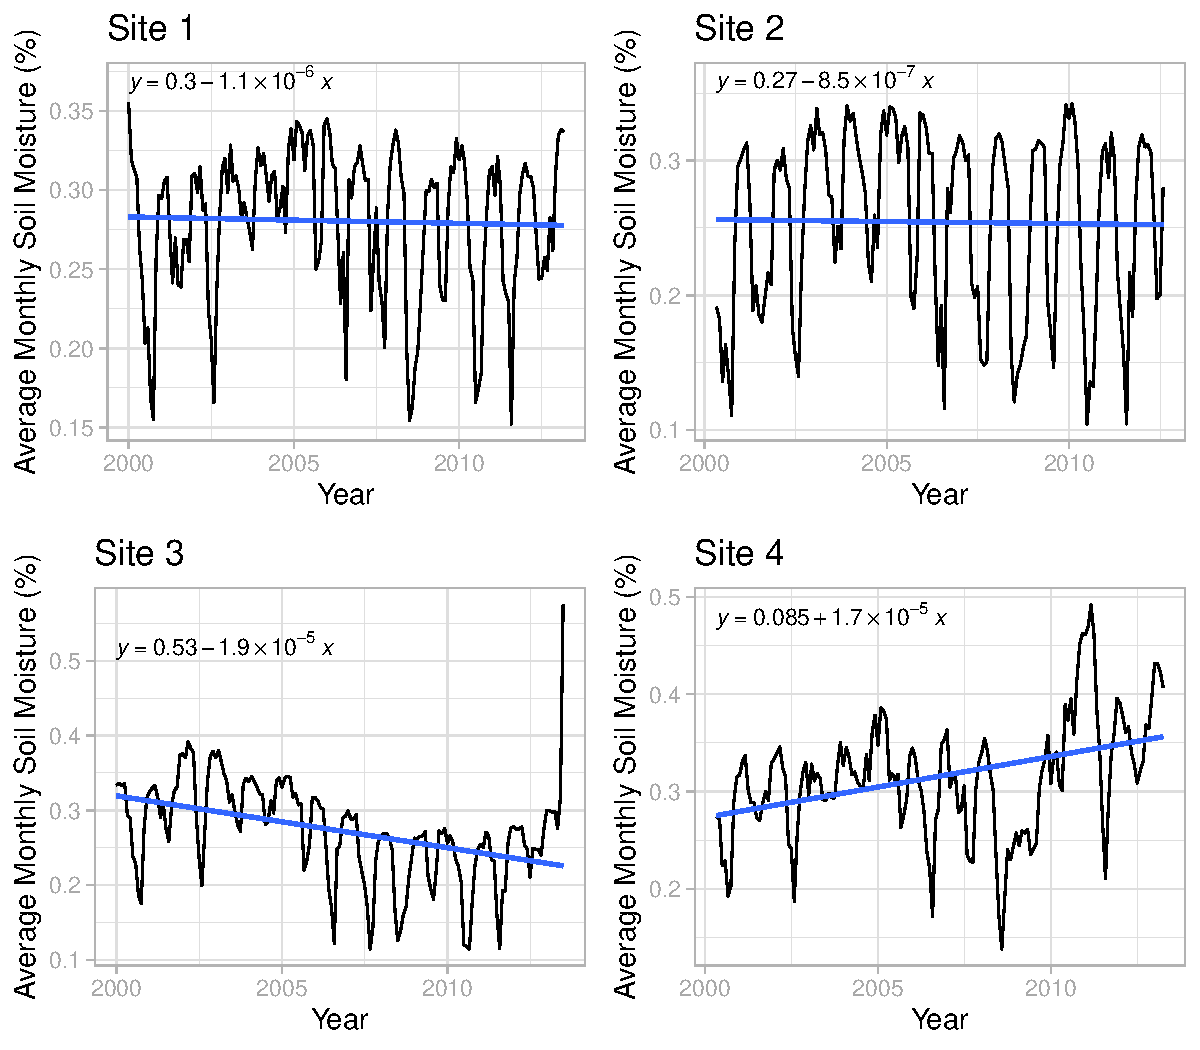
\includegraphics{Project_Template_files/figure-latex/Average Monthly Soil Moisture Cowplot-1.pdf}
\caption{Average Monthly Soil Moisture}
\end{figure}

\begin{figure}
\centering
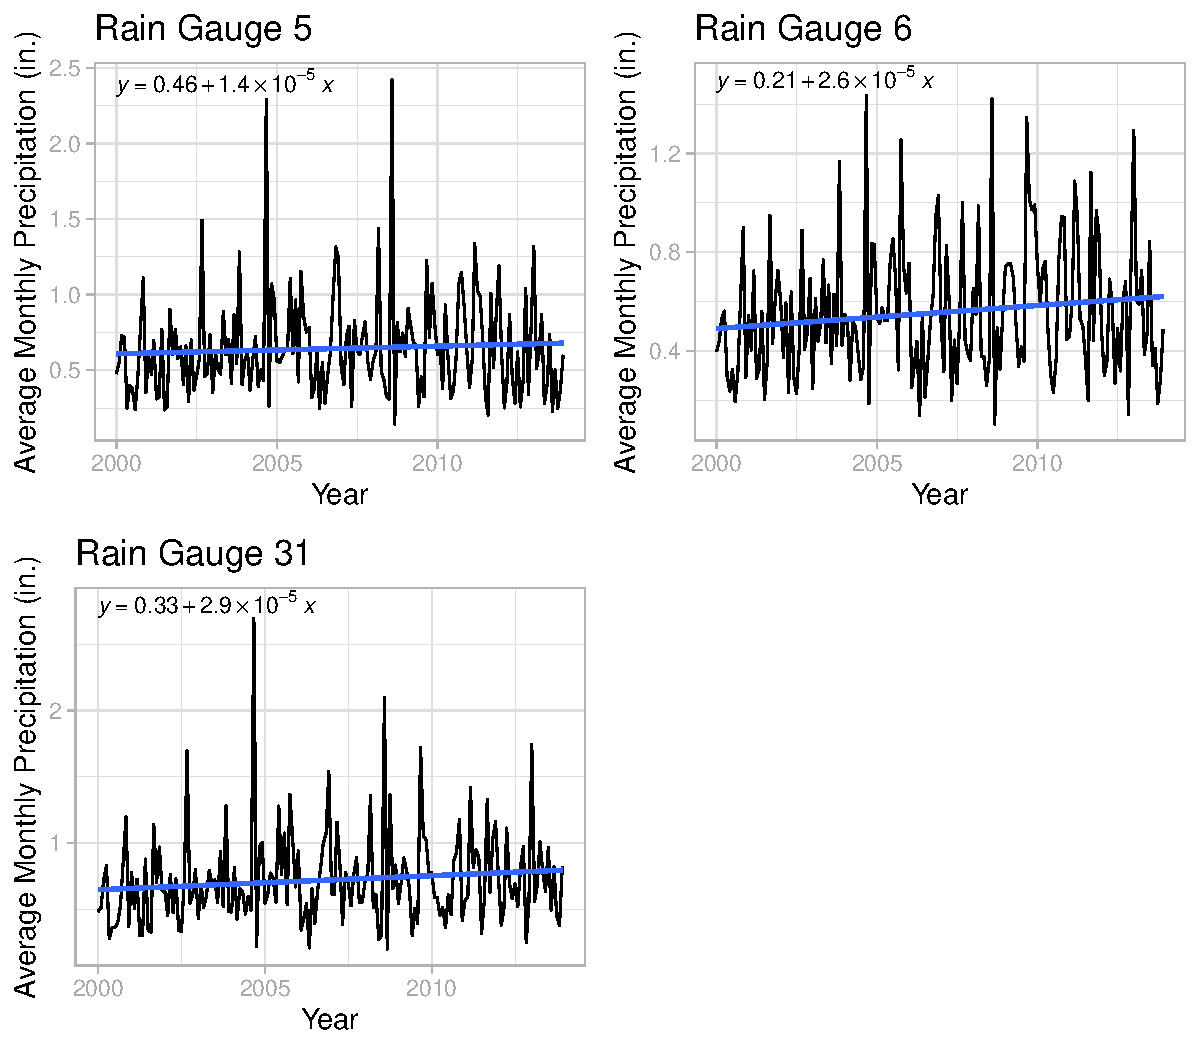
\includegraphics{Project_Template_files/figure-latex/Average Monthly Precipitation Cowplot-1.pdf}
\caption{Average Monthly Precipitation}
\end{figure}

\begin{figure}
\centering
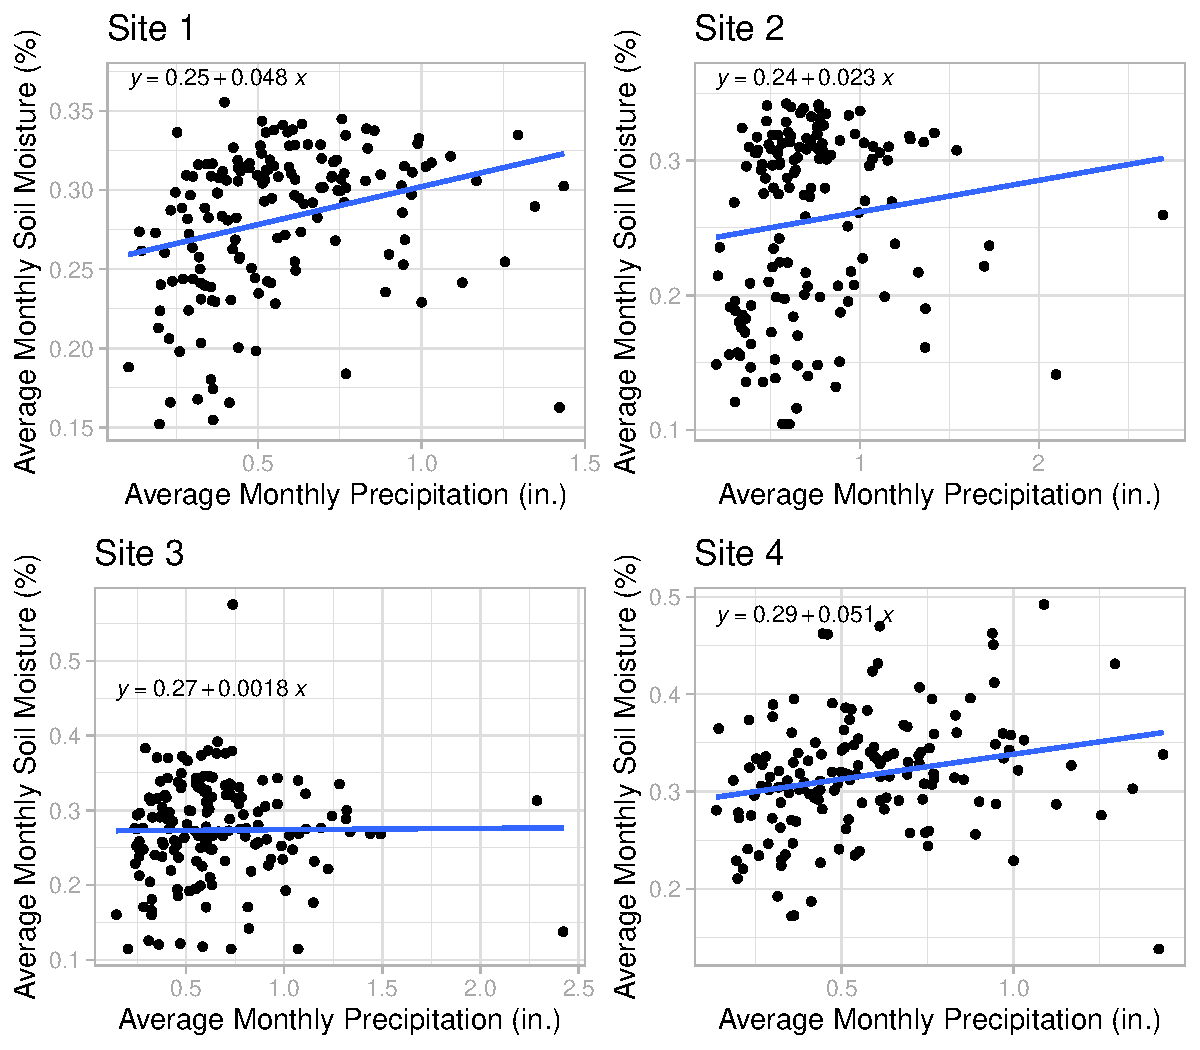
\includegraphics{Project_Template_files/figure-latex/Average Monthly Soil Moisture and Precipitation Cowplot-1.pdf}
\caption{Average monthly soil moisture and precipitation}
\end{figure}

\newpage

\hypertarget{analysis}{%
\section{Analysis}\label{analysis}}

\hypertarget{question-1-has-soil-moisture-in-the-upper-30-centimeters-of-soil-increased-or-decreased-in-coweeta-basin-from-2000-to-2013-at-each-of-the-four-research-sites}{%
\subsection{Question 1: Has soil moisture in the upper 30 centimeters of
soil increased or decreased in Coweeta Basin from 2000 to 2013 at each
of the four research
sites?}\label{question-1-has-soil-moisture-in-the-upper-30-centimeters-of-soil-increased-or-decreased-in-coweeta-basin-from-2000-to-2013-at-each-of-the-four-research-sites}}

\hypertarget{question-2-which-sites-experienced-the-greatest-change-in-soil-moisture-over-time}{%
\subsection{Question 2: Which sites experienced the greatest change in
soil moisture over
time?}\label{question-2-which-sites-experienced-the-greatest-change-in-soil-moisture-over-time}}

\hypertarget{question-3-what-is-the-impact-of-elevation-on-soil-moisture}{%
\subsection{Question 3: What is the impact of elevation on soil
moisture?}\label{question-3-what-is-the-impact-of-elevation-on-soil-moisture}}

In order to analyze potential changes in soil moisture in the upper 30
cm in Coweeta Basin from 2000 to 2013 at each of the four research
sites, we completed a time series analysis (TSA) of monthly soil
moisture for each site. TSA is used to track a response variable over
time to understand whether an increasing or decreasing trend exists
across a given time period. Our time series model tracked time in months
as the explanatory variable and soil moisture expressed as percent water
content as the response variable. TSA can be broken down into the
following four components: (1) seasonal component, (2) trend component,
(3) error or random component, and (4) cyclical component. For the
purpose of our analysis, we focused on the seasonal and trend components
in order to interpret general tendencies and repeating cycles,
i.e.~seasonality. After decomposing and plotting the time series, we
compared the length of the gray bars to the right of each plot that
explain the relative scale of each component. A longer bar corresponds
to smaller variability of that component in the dataset whereas a
smaller bar corresponds to larger variability of that component in the
dataset. As a result, the trend component explained most of the
variability in the dataset of sites 3 and 4 and the seasonality
component explained most of the variability in the dataset of sites 1
and 2.

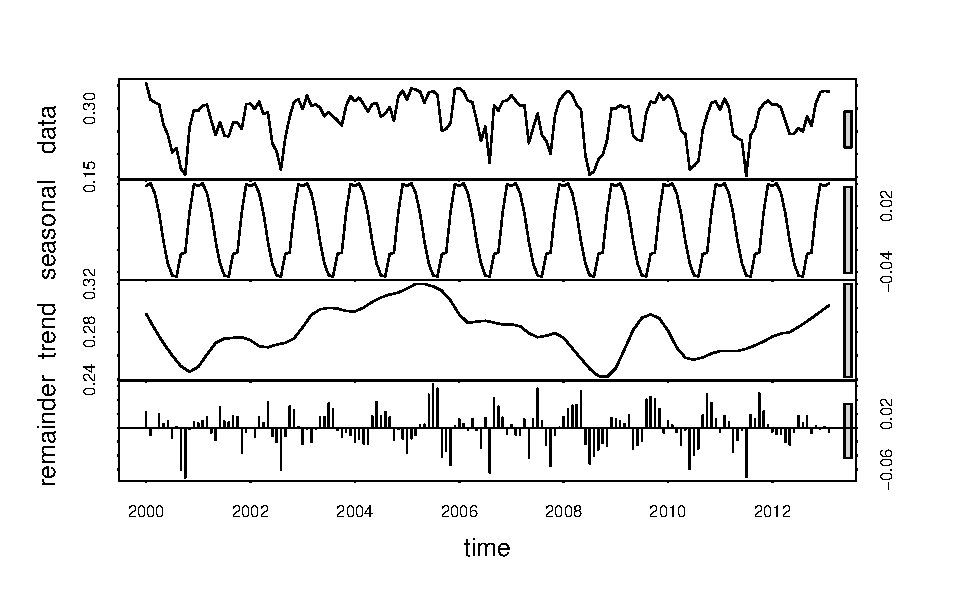
\includegraphics{Project_Template_files/figure-latex/TSA-1.pdf}
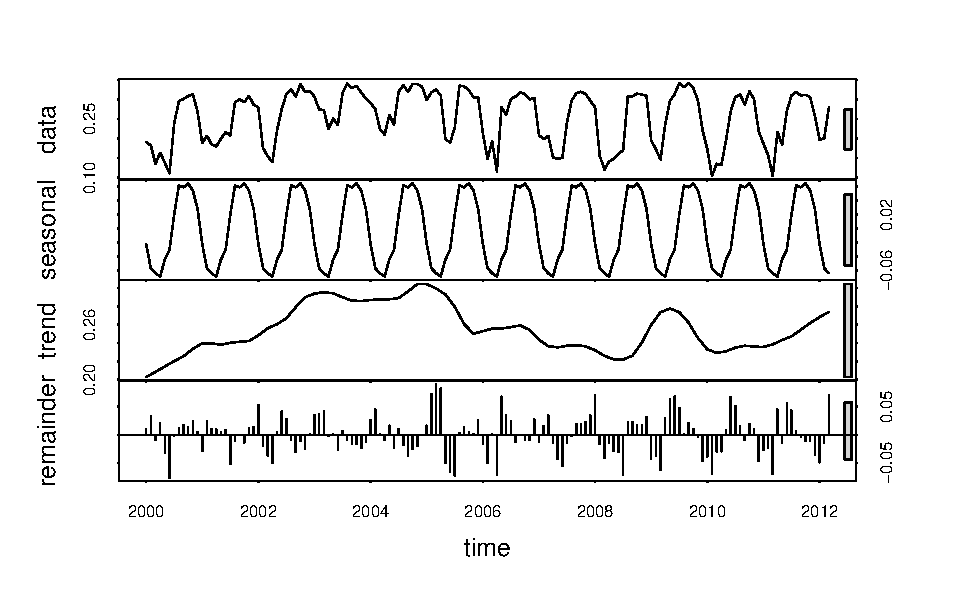
\includegraphics{Project_Template_files/figure-latex/TSA-2.pdf}
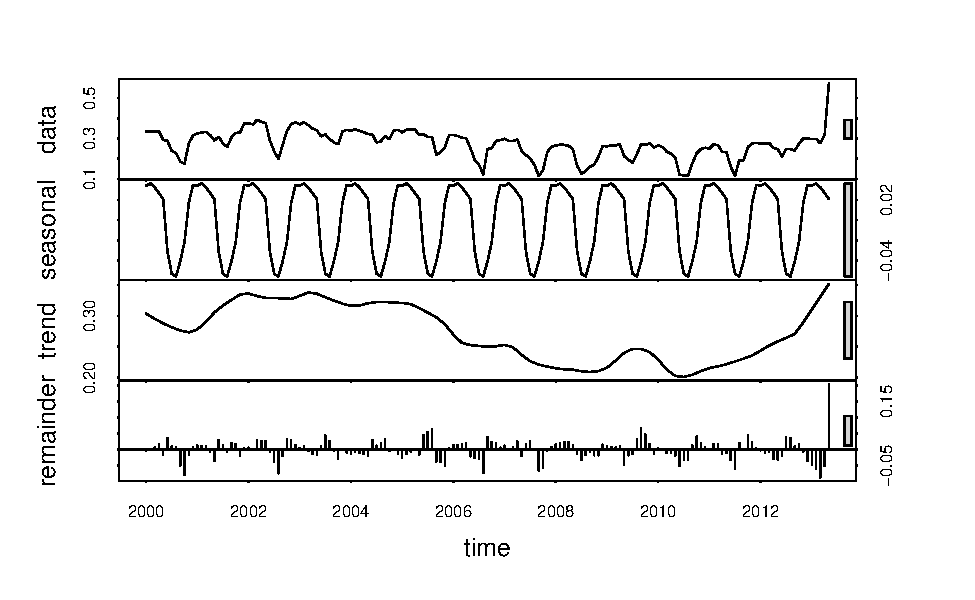
\includegraphics{Project_Template_files/figure-latex/TSA-3.pdf}
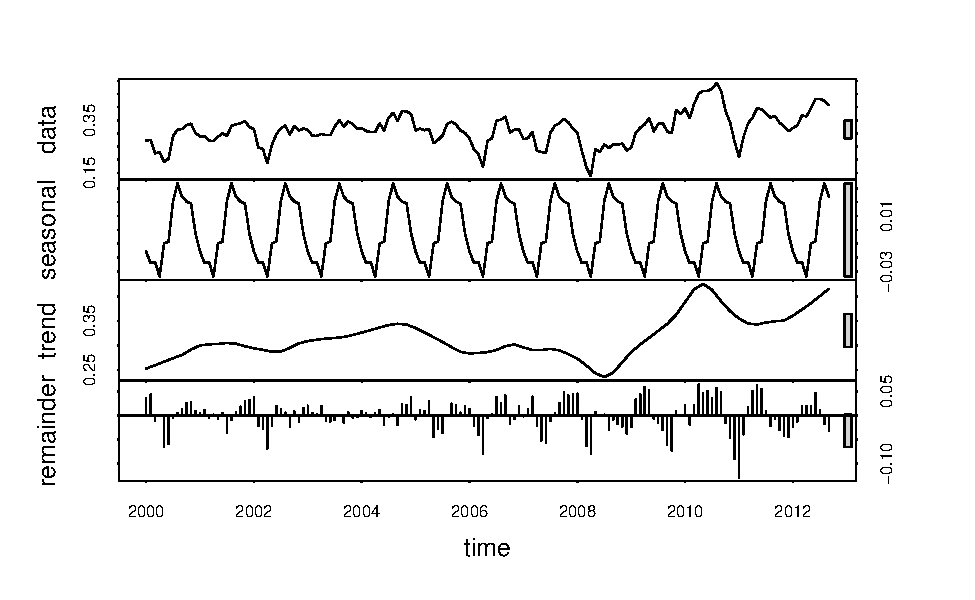
\includegraphics{Project_Template_files/figure-latex/TSA-4.pdf}

We also conducted a Seasonal Mann-Kendall trend analysis of monthly soil
moisture for each research site in order to identify seasonal trends in
the data. The Seasonal Mann-Kendall trend analysis is a type of
monotonic trend analysis test that is non-parametric and can be used on
seasonal data that exhibits a repeating pattern at regular intervals
over time. A monotonic trend is defined as a gradual change over time
that is uniform in direction. The results of the Seasonal Mann-Kendall
are as follows:

\begin{itemize}
\tightlist
\item
  \emph{Site 1}: p-value = 0.80898
\item
  \emph{Site 2}: p-value = 0.35739
\item
  \emph{Site 3}: p-value = 3.2565e-12
\item
  \emph{Site 4}: p-value = 1.0157e-5
\end{itemize}

A p-value less than 0.05 means we must reject the null hypothesis that
states the data is stationary and conclude that there is a statistically
significant trend in average monthly soil moisture. A p-value greater
than 0.05 means we fail to reject the null hypothesis that states the
data is stationary and conclude there is not a statistically significant
trend in average monthly soil moisture. In reference to the p-values
above, sites 1 and 2 have a p-value greater than 0.05 which is not
statistically significant. However, sites 3 and 4 have a p-value less
than 0.05 which means there is a statistically significant trend at
these sites.

\begin{Shaded}
\begin{Highlighting}[]
\CommentTok{\#Running the Seasonal Mann{-}Kendall trend analysis of average monthly soil moisture}
\NormalTok{site1\_trend }\OtherTok{\textless{}{-}}\NormalTok{ Kendall}\SpecialCharTok{::}\FunctionTok{SeasonalMannKendall}\NormalTok{(site1\_ts)}
\FunctionTok{summary}\NormalTok{(site1\_trend)}

\NormalTok{site2\_trend }\OtherTok{\textless{}{-}}\NormalTok{ Kendall}\SpecialCharTok{::}\FunctionTok{SeasonalMannKendall}\NormalTok{(site2\_ts)}
\FunctionTok{summary}\NormalTok{(site2\_trend)}

\NormalTok{site3\_trend }\OtherTok{\textless{}{-}}\NormalTok{ Kendall}\SpecialCharTok{::}\FunctionTok{SeasonalMannKendall}\NormalTok{(site3\_ts)}
\FunctionTok{summary}\NormalTok{(site3\_trend)}

\NormalTok{site4\_trend }\OtherTok{\textless{}{-}}\NormalTok{ Kendall}\SpecialCharTok{::}\FunctionTok{SeasonalMannKendall}\NormalTok{(site4\_ts)}
\FunctionTok{summary}\NormalTok{(site4\_trend)}
\end{Highlighting}
\end{Shaded}

\hypertarget{question-4-is-there-a-relationship-between-soil-moisture-and-precipitation-that-can-be-observed-at-these-four-research-sites}{%
\subsection{Question 4: Is there a relationship between soil moisture
and precipitation that can be observed at these four research
sites?}\label{question-4-is-there-a-relationship-between-soil-moisture-and-precipitation-that-can-be-observed-at-these-four-research-sites}}

Lastly, we utilized a simple linear regression to determine the strength
of the statistical relationship between monthly precipitation and soil
moisture. Regression is the fitting of a line to a set of data points
and a simple linear regression explains the linear relationship between
two variables. The two outputs of the linear model that we chose to
focus on were the p-value and multiple R-squared, or coefficient of
determination, which is a measure of the percentage of variability in
the values of average monthly precipitation (response variable) that is
explained by average monthly soil moisture (explanatory variable) and
ranges from 0 to 1. The results of the simple linear regression are as
follows:

\begin{itemize}
\tightlist
\item
  \emph{Site 1}:

  \begin{itemize}
  \tightlist
  \item
    p-value = 0.0003247
  \item
    Multiple R-squared = 0.08024
  \end{itemize}
\item
  \emph{Site 2}:

  \begin{itemize}
  \tightlist
  \item
    p-value = 0.127
  \item
    Multiple R-squared = 0.0161
  \end{itemize}
\item
  \emph{Site 3}:

  \begin{itemize}
  \tightlist
  \item
    p-value = 0.9118
  \item
    Multiple R-squared = 7.783e-5
  \end{itemize}
\item
  \emph{Site 4}:

  \begin{itemize}
  \tightlist
  \item
    p-value = 0.00392
  \item
    Multiple R-squared = 0.05413
  \end{itemize}
\end{itemize}

A p-value less than 0.05 means we must reject the null hypothesis that
assumes there is no relationship or correlation between average monthly
soil moisture and precipitation and conclude there is a statistically
significant relationship between the two variables. A p-value greater
than 0.05 means we fail to reject the null hypothesis and conclude there
is not a statistically significant relationship between the two
variables. In reference to the p-values above, sites 1 and 4 have a
significant relationship between average monthly soil moisture and
precipitation while sites 2 and 3 do not have a significant relationship
between the two variables. Additionally, site 1 had the highest
R-squared value of 0.08024 which indicates that approximately 8.02\% of
the variability in average monthly soil moisture is explained by average
monthly precipitation, followed by site 4, site 2, and site 3 in
decreasing value. Reviewing the slopes of the linear model for each site
also emphasizes the strongest relationship between soil moisture and
precipitation at sites 1 and 4 with soil moisture expected to increase
approximately 4.79\% for every 1 inch increase in precipitation at site
1 and approximately 5.11\% for every 1 inch increase in precipitation at
site 4.

\begin{Shaded}
\begin{Highlighting}[]
\CommentTok{\#Running a linear model to determine the strength of the statistical relationship between precipitation and soil moisture}
\NormalTok{lm\_site1 }\OtherTok{\textless{}{-}} \FunctionTok{lm}\NormalTok{(}\AttributeTok{data =}\NormalTok{ site1\_soil\_precip, }\AttributeTok{formula =}\NormalTok{ AverageMonthlySmois30 }\SpecialCharTok{\textasciitilde{}}\NormalTok{ AverageMonthlyPrecip)}
\FunctionTok{summary}\NormalTok{(lm\_site1)}

\NormalTok{lm\_site2 }\OtherTok{\textless{}{-}} \FunctionTok{lm}\NormalTok{(}\AttributeTok{data =}\NormalTok{ site2\_soil\_precip, }\AttributeTok{formula =}\NormalTok{ AverageMonthlySmois30 }\SpecialCharTok{\textasciitilde{}}\NormalTok{ AverageMonthlyPrecip)}
\FunctionTok{summary}\NormalTok{(lm\_site2)}

\NormalTok{lm\_site3 }\OtherTok{\textless{}{-}} \FunctionTok{lm}\NormalTok{(}\AttributeTok{data =}\NormalTok{ site3\_soil\_precip, }\AttributeTok{formula =}\NormalTok{ AverageMonthlySmois30 }\SpecialCharTok{\textasciitilde{}}\NormalTok{ AverageMonthlyPrecip)}
\FunctionTok{summary}\NormalTok{(lm\_site3)}

\NormalTok{lm\_site4 }\OtherTok{\textless{}{-}} \FunctionTok{lm}\NormalTok{(}\AttributeTok{data =}\NormalTok{ site4\_soil\_precip, }\AttributeTok{formula =}\NormalTok{ AverageMonthlySmois30 }\SpecialCharTok{\textasciitilde{}}\NormalTok{ AverageMonthlyPrecip)}
\FunctionTok{summary}\NormalTok{(lm\_site4)}
\end{Highlighting}
\end{Shaded}

\newpage

\hypertarget{summary-and-conclusions}{%
\section{Summary and Conclusions}\label{summary-and-conclusions}}

In analyzing the results of these statistical tests, we are able to draw
conclusions on soil moisture trends and determine correlation between
soil moisture and precipitation from 2000 to 2013 in Coweeta Basin. Our
main research question focused on identifying an increasing or
decreasing trend in soil moisture in the upper 30 cm at each of the four
research sites from 2000 to 2013. The results of the time series
analysis and Seasonal Mann-Kendall test indicate that there is a
statistically significant trend at sites 3 and 4, with the trend
component explaining much of the variability in the dataset of sites 3
and 4 and the seasonality component explaining much of the variability
in the dataset of sites 1 and 2. Viewing the plot of average monthly
soil moisture over time also provides insight on these trends. Sites 1,
2, and 3 have a decreasing trend in average monthly soil moisture as
indicated by a negative slope whereas site 4 has an increasing trend in
average monthly soil moisture as indicated by the positive slope. In
comparing these trends to determine which sites experienced the greatest
change in soil moisture over time, the results of the Seasonal
Mann-Kendall test conclude that sites 3 and 4 have the strongest trend
in average monthly soil moisture. However, the directionality of these
trends differ with a decreasing trend at site 3 and an increasing trend
at site 4.

Additional questions that we explored include the impact of elevation on
soil moisture as well as the relationship between soil moisture and
precipitation at each of the four research sites. Sites 2 and 3 had the
highest elevations at approximately 1380 meters and 1215 meters,
respectively. Sites 1 and 4 had the lowest elevations at approximately
817 meters and 735 meters, respectively. The results of the Seasonal
Mann-Kendall test emphasize a significant trend present at site 4 which
is the lowest elevation of all four sites. While an increasing trend of
average monthly soil moisture exists at this site, the test also
determines that there is not a significant trend at sites 1 or 2. As a
result, we are unable to definitively conclude the impact of elevation
on soil moisture. In order to address the relationship between soil
moisture and precipitation, the results of the linear regression
indicated that sites 1 and 4 have a statistically significant
relationship between average monthly soil moisture and precipitation.
Site 1 had the strongest relationship between the two variables as
indicated by the highest R-squared value while site 3 had the weakest
relationship as indicated by the smallest R-squared value. In reviewing
these conclusions, we do acknowledge that the location of rain gauges
and soil moisture sites paired in this study may be a possible
limitation or shortcoming. Although the pairing of soil moisture sites
and rain gauge stations was based on closest proximity via geographic
coordinates, there is uncertainty of local topography in these regions
that may lead to slight distortions in the analysis of the relationship
between average monthly soil moisture and precipitation.

\newpage

\hypertarget{references}{%
\section{References}\label{references}}

SRS Science Communications. ``Forest Watershed Science Coweeta
Hydrologic Laboratory.'' USDA - U.S. Forest Service - Southern Research
Station, \url{https://www.srs.fs.usda.gov/coweeta/}.

\end{document}
